\chapter{Skrypt symulacji}
\begin{figure}[tp]
    \centering
    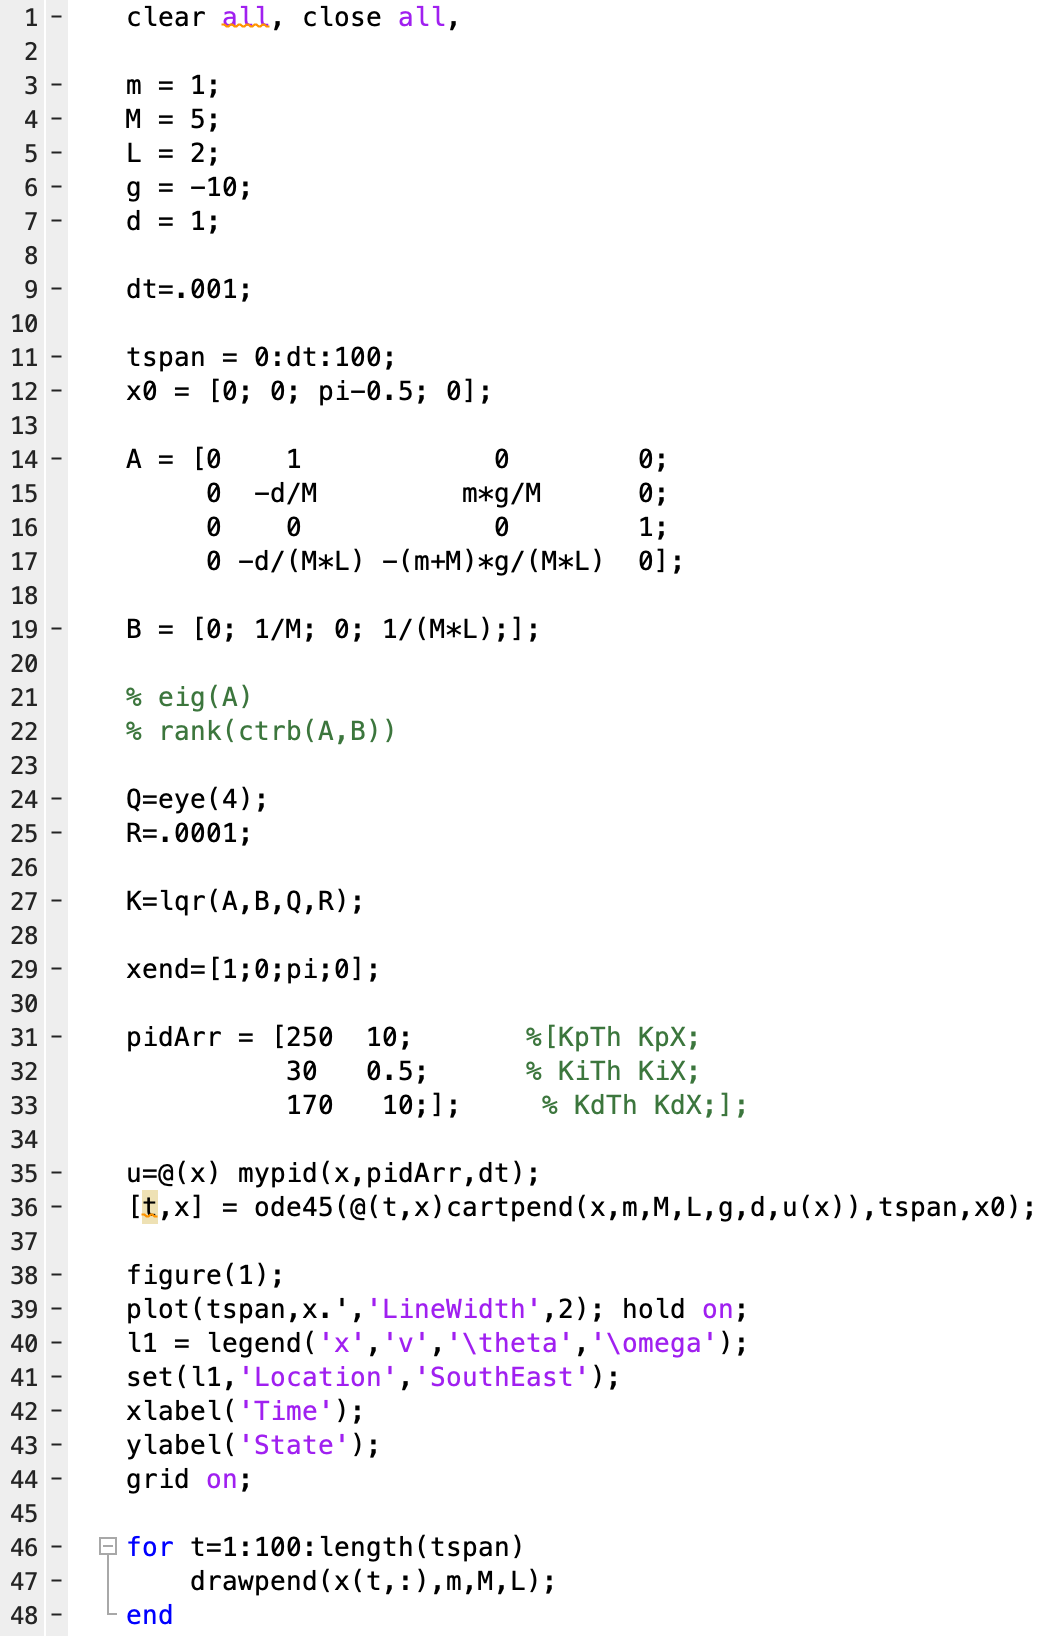
\includegraphics[height=\textheight]{praca_dyplomowa/figures/simpend.png}
    \caption{Główny skrypt symulacji}
    \label{fig:simpend}
\end{figure}

\begin{figure}
    \centering
    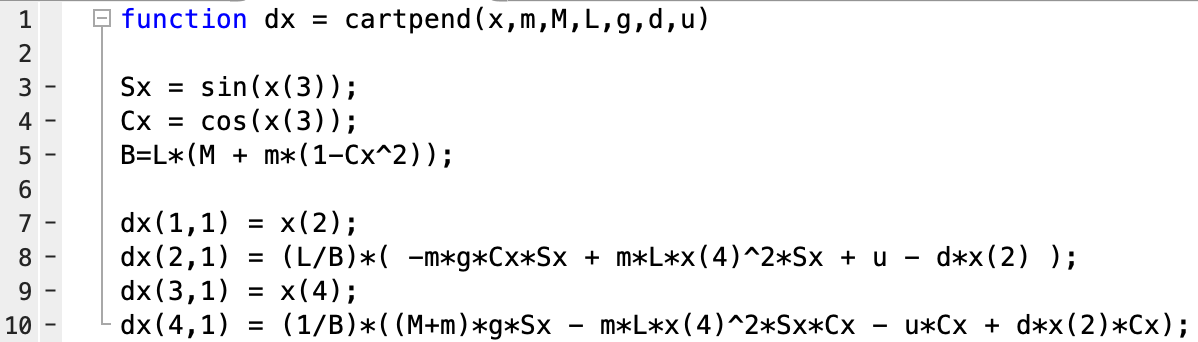
\includegraphics[width=\textwidth]{praca_dyplomowa/figures/cartpend.png}
    \caption{Funkcja \textit{cartpend}}
    \label{fig:cartpend}
\end{figure}

\begin{figure}
    \centering
    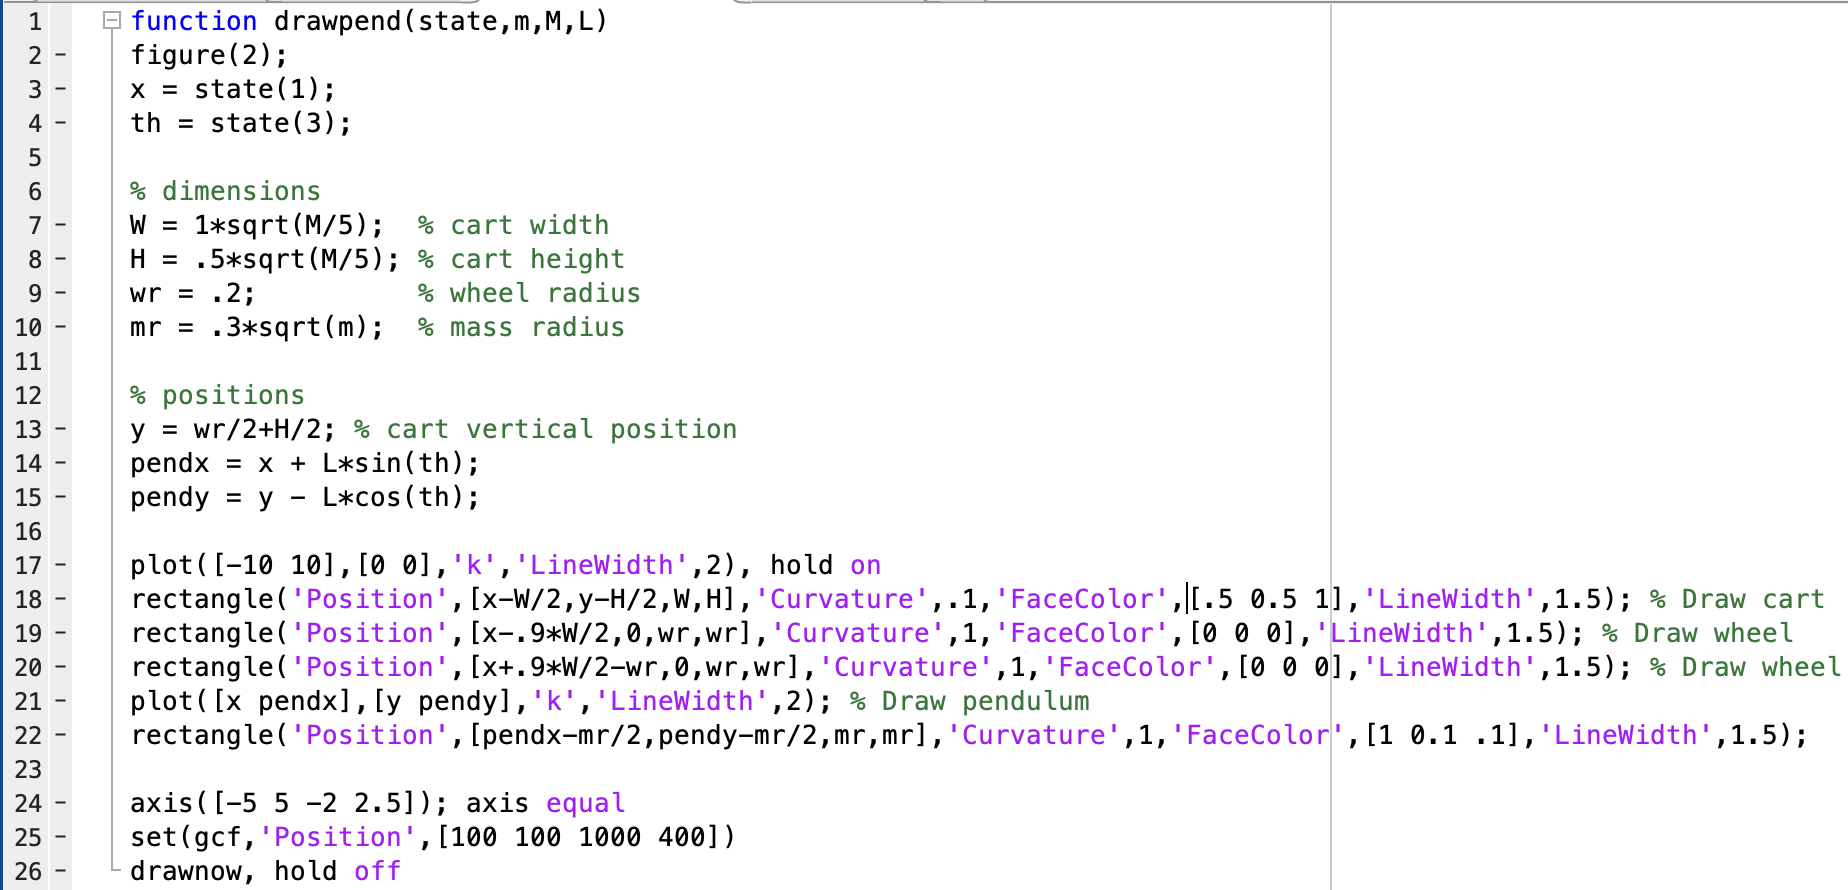
\includegraphics[width=\textwidth]{praca_dyplomowa/figures/drawpend.png}
    \caption{Funkcja \textit{drawpend}}
    \label{fig:drawpend}
\end{figure}

\begin{figure}
    \centering
    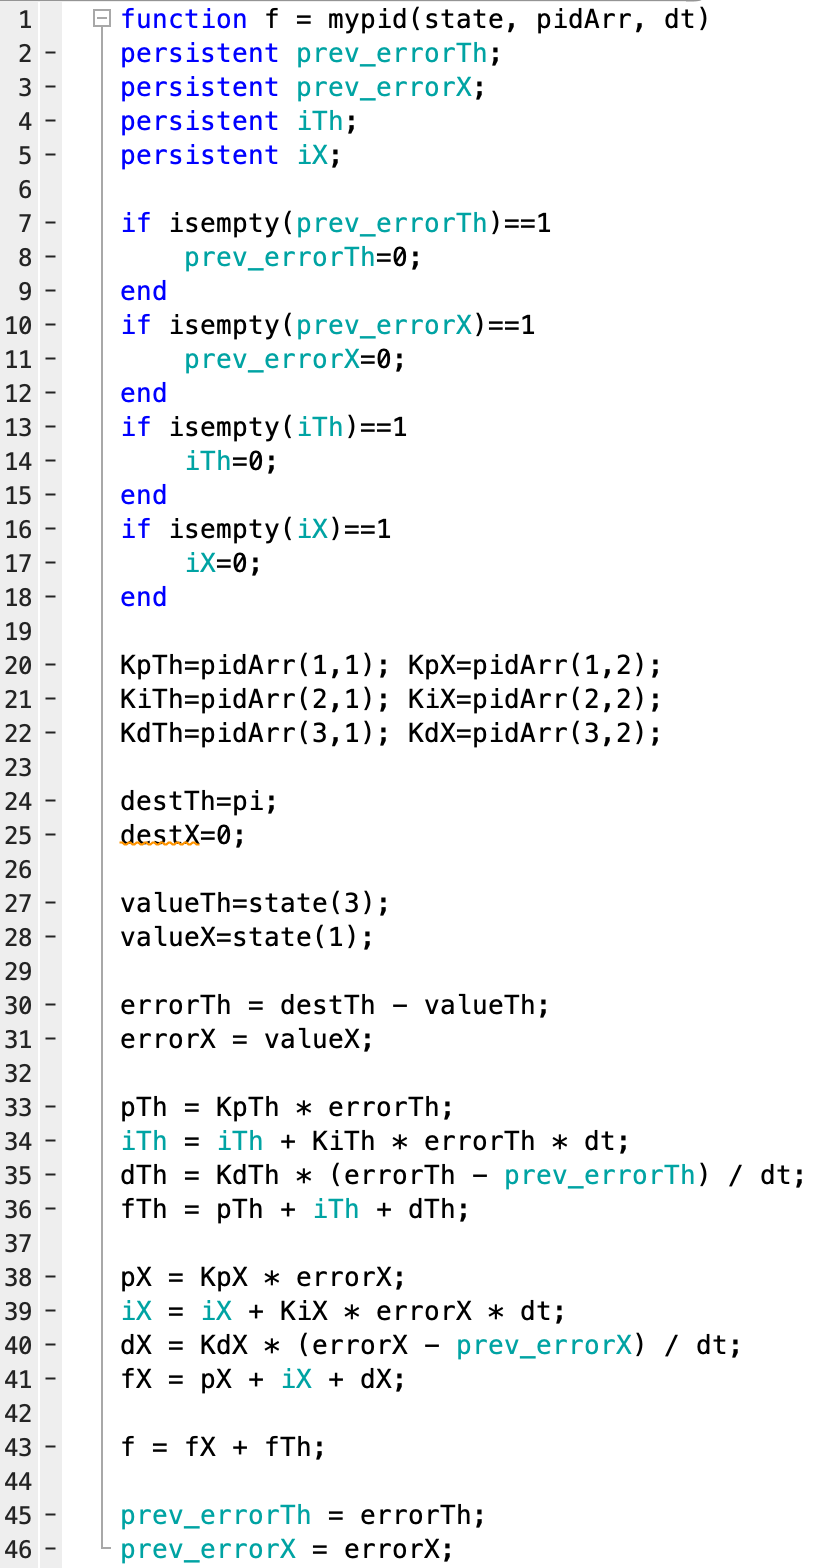
\includegraphics[height=\textheight]{praca_dyplomowa/figures/mypid.png}
    \caption{Funkcja \textit{mypid}}
    \label{fig:mypid}
\end{figure}

\begin{figure}
    \centering
    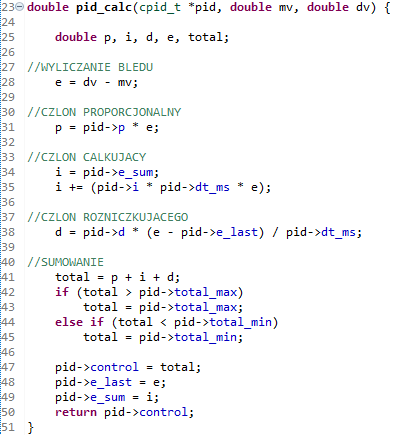
\includegraphics[width=\textwidth]{praca_dyplomowa/figures/pidkod.png}
    \caption{Algorytm regulatora \textit{PID IND}}
    \label{fig:pidind}
\end{figure}